\newpage
\section{Metodologia Experimental}

\subsection{Materiais}
O material utilizado foi:
\begin{itemize}
\item Computador.
\item Software Orcad.
\item Software MATLAB.

\end{itemize}
Para execução do experimento, faz-se necessário executar os seguintes passos (com base no circuito da figura \ref{f_sch}:

\begin{itemize}

\item simular o circuito mostrado na figura \ref{f_sch} com o software Orcad;
\item analisar a forma de onda de saída (frequência, amplitude, distorção);
\item adicionar uma resistência de 10M $\Omega$ em paralelo com uma capacitância de 10pF a saída, de modo a simular uma ponteira de osciloscópio;
\item verificar se a frequência de saída é modificada pela ponteira de osciloscópio;
\item variar a tensão de saída em +- 20\% e verificar se há alteração na frequência de saída;
\item calcular a estabilidade relativa em partes por milhão [ppm] para a variação de tensão.
\item analisar as harmônicas geradas pelo circuito.
\end{itemize}

\begin{figure}[H]
\centering
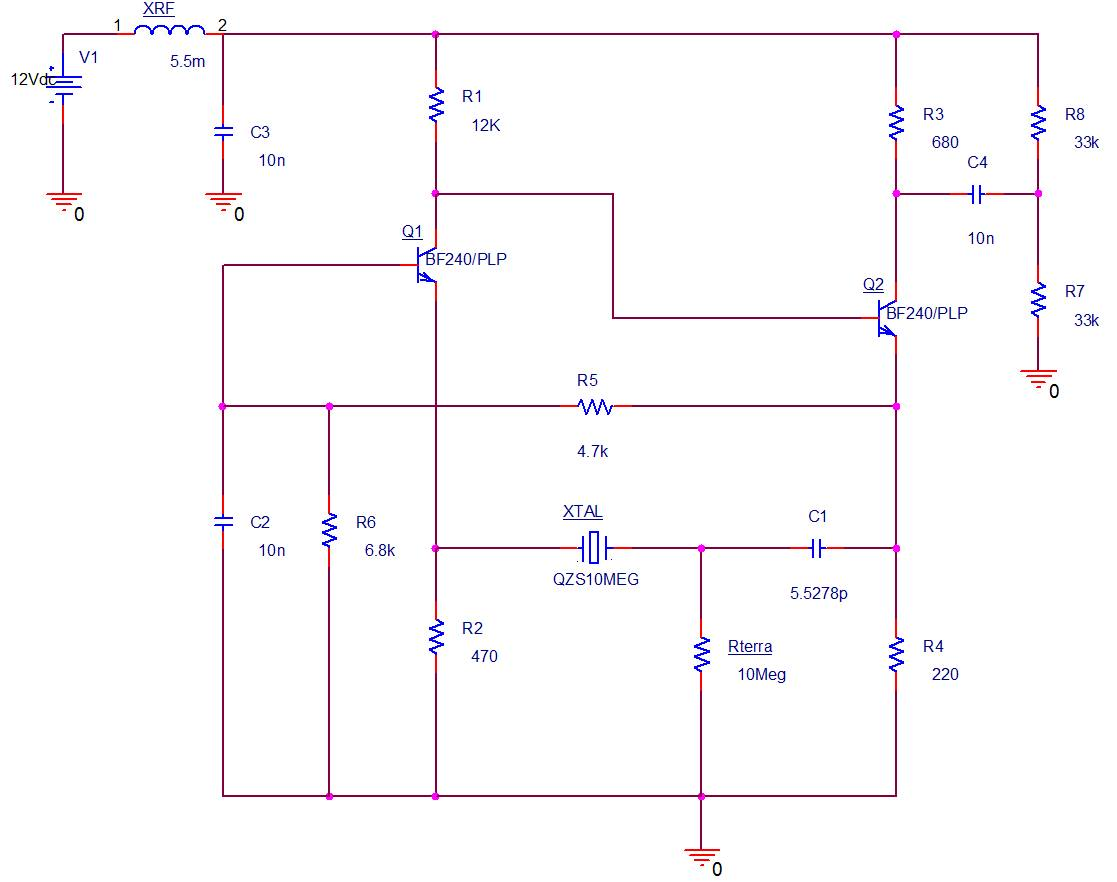
\includegraphics[scale=0.3]{Imagens/sch.jpg}
\caption{Oscilador a crital.}
\label{f_sch}
\end{figure}
